\documentclass[a4paper,12pt]{article}
\usepackage{graphicx}
\usepackage{epstopdf}
\usepackage{gensymb}
%% Definitioner för LIPS-dokument

\usepackage[swedish]{babel}
\usepackage[utf8]{inputenc}
\usepackage[T1]{fontenc}
\usepackage{times}
\usepackage{ifthen}

\usepackage[margin=25mm]{geometry}

\usepackage{fancyhdr}
\pagestyle{fancy}
\lhead{}
\chead{\textbf{\LIPSprojekttitel}}
\rhead{\textbf{\textsl{LiTH}}\\\textbf{\LIPSdatum}}
\lfoot{\textbf{\LIPSkursnamn}\\\textbf{\LIPSdokumentansvarig}}
\cfoot{\textbf{\LIPSprojektgrupp}\\\textbf{\LIPSgruppepost}}
\rfoot{\textbf{\textsc{Lip}s}\\\textbf{Sida~\thepage}}

\setlength{\parindent}{0pt}
\setlength{\parskip}{1ex plus 0.5ex minus 0.2ex}


\newcommand{\twodigit}[1]{\ifthenelse{#1<10}{0}{}{#1}}
\newcommand{\dagensdatum}{\number\year-\twodigit{\number\month}-\twodigit{\number\day}}

%% ------------------------------------------
% NYBILD
% Skapar centrerad bild med caption
%   
% #1: Filens url relativt '/bilder/'
% #2:  Caption
% #3: Label
% #4: Skalning
%% ------------------------------------------
\newcommand{\nyBild}[4] 
{\begin{figure}[H]
  \centering
 \includegraphics[angle=0,scale=#4]{bilder/#1}
  \caption{#2}
  \label{fig:#3}
\end{figure}}



%%  Redefinitions of commands containing @
\makeatletter
\makeatother

\newcommand{\LIPStitelsida}{%
{\ }\vspace{45mm}
\begin{center}
  \textbf{\Huge \LIPSdokumenttyp}
\end{center}
\begin{center}
  {\Large Redaktör: \LIPSredaktor}
\end{center}
\begin{center}
  {\Large \textbf{Version \LIPSversion}}
\end{center}
\vfill
\begin{center}
  {\large Status}\\[1.5ex]
  \begin{tabular}{|*{3}{p{40mm}|}}
    \hline
    Granskad & \LIPSgranskare & \LIPSgranskatdatum \\
    \hline
    Godkänd & \LIPSgodkannare & \LIPSgodkantdatum \\
    \hline
  \end{tabular}
\end{center}
\newpage
}


\newenvironment{LIPSprojektidentitet}{%
{\ }\vspace{45mm}
\begin{center}
  {\Large PROJEKTIDENTITET}\\[0.5ex]
  {\small
  \LIPSartaltermin, \LIPSprojektgrupp\\
  Linköpings Tekniska Högskola, ISY
  }
\end{center}
\begin{center}
  {\small Gruppdeltagare}\\
%  \begin{tabular}{|p{30mm}|p{40mm}|p{35mm}|p{45mm}|}
  \begin{tabular}{|l|p{45mm}|p{25mm}|l|}
    \hline
    \textbf{Namn} & \textbf{Ansvar} & \textbf{Telefon} & \textbf{E-post} \\
    \hline
}%
{%
    \hline
  \end{tabular}
\end{center}
\begin{center}
  {\small
    \textbf{E-postlista för hela gruppen}: \LIPSgruppepost\\
    \textbf{Hemsida}: \LIPSgrupphemsida\\[1ex]
    \textbf{Kund}: \LIPSkund\\
    \textbf{Kontaktperson hos kund}: \LIPSkundkontakt\\
    \textbf{Kursansvarig}: \LIPSkursansvarig\\
    \textbf{Handledare}: \LIPShandledare\\
  }
\end{center}
\newpage
}
\newcommand{\LIPSgruppmedlem}[4]{\hline {#1} & {#2} & {#3} & {#4} \\}



\newenvironment{LIPSdokumenthistorik}{%
\begin{center}
  Dokumenthistorik\\[1ex]
  \begin{small}
    \begin{tabular}{|l|l|p{60mm}|l|l|}
      \hline
      \textbf{Version} & \textbf{Datum} & \textbf{Utförda förändringar} & \textbf{Utförda av} & \textbf{Granskad} \\
      }%
    {%
      \hline
    \end{tabular}
  \end{small}
\end{center}
}
\newcommand{\LIPSversionsinfo}[5]{\hline {#1} & {#2} & {#3} & {#4} & {#5} \\}

\newcounter{LIPSkravnummer}
\newcounter{LIPSunderkravnummer}[LIPSkravnummer]
\newenvironment{LIPSkravlista}{%
  \begin{tabular}{|p{25mm}|p{25mm}|p{85mm}|p{5mm}|}
    }%
  {%
    \hline
  \end{tabular}
}
\newcommand{\LIPSkrav}[3]{\hline\stepcounter{LIPSkravnummer}\textbf{Krav nr \arabic{LIPSkravnummer}} & \textbf{{#1}} & {#2} & \textbf{{#3}} \\}
\newcommand{\LIPSunderkrav}[3]{\hline\stepcounter{LIPSunderkravnummer}\textbf{Krav nr \arabic{LIPSkravnummer}\Alph{LIPSunderkravnummer}} & \textbf{{#1}} & {#2} & \textbf{{#3}} \\}





%%% Local Variables: 
%%% mode: latex
%%% TeX-master: "kravspec_mall"
%%% End: 



\newcommand{\LIPSartaltermin}{2012/VT}
\newcommand{\LIPSkursnamn}{TSEA27}

\newcommand{\LIPSprojekttitel}{Komborobot}

\newcommand{\LIPSprojektgrupp}{Grupp 17}
\newcommand{\LIPSgruppepost}{komborobot@googlegroups.com}
\newcommand{\LIPSgrupphemsida}{finns ej}
\newcommand{\LIPSdokumentansvarig}{Mattias Jansson}

\newcommand{\LIPSkund}{ISY, Linköpings universitet, 581\,83 Linköping}
\newcommand{\LIPSkundkontakt}{Tomas Svensson, 013-281368, tomass@isy.liu.se}
\newcommand{\LIPSkursansvarig}{Tomas Svensson, 013-281368, tomass@isy.liu.se}
\newcommand{\LIPShandledare}{}


\newcommand{\LIPSdokumenttyp}{Systemskiss}
\newcommand{\LIPSredaktor}{Simon Larsson}
\newcommand{\LIPSversion}{0.1}
\newcommand{\LIPSdatum}{\dagensdatum}

\newcommand{\LIPSgranskare}{}
\newcommand{\LIPSgranskatdatum}{}
\newcommand{\LIPSgodkannare}{}
\newcommand{\LIPSgodkantdatum}{}

\begin{document}

\LIPStitelsida

%% Argument till \LIPSgruppmedlem: namn, roll i gruppen, telefonnummer, epost
\begin{LIPSprojektidentitet}
  \LIPSgruppmedlem{Simon Larsson}{Projektledare (PL)}{070-7311646}{simla804@student.liu.se}
  \LIPSgruppmedlem{\LIPSdokumentansvarig}{Dokumentansvarig (DOK)}{073-6837074}{matja307@student.liu.se}
  \LIPSgruppmedlem{Gustav Svensk}{Reglersystem (REG)}{073-6208776}{gussv666@student.liu.se}
  \LIPSgruppmedlem{Johan Jönsson}{Mjukvara (KA)}{073-8305758}{johjo939@student.liu.se}
  \LIPSgruppmedlem{Tobias Andersson}{Hårdvara (HV)}{073-7201098}{toban963@student.liu.se}
  \LIPSgruppmedlem{Markus Falck}{Leveransansvarig (LV)}{076-3457552}{marlo265@student.liu.se}
  \LIPSgruppmedlem{Simon Wallin}{Testansvarig (GM)}{076-2300665}{simwa252@student.liu.se}
\end{LIPSprojektidentitet}

\tableofcontents{}
\newpage

%% Argument till \LIPSversionsinfo: versionsnummer, datum, ändringar, utfört av, granskat av
\addcontentsline{toc}{section}{Dokumenthistorik}
\begin{LIPSdokumenthistorik}
  \LIPSversionsinfo{1.0}{2012-02-23}{Första versionen}{gussv666}{johjo939}
  \LIPSversionsinfo{0.1}{2012-02-10}{Första utkast.}{gussv666}{johjo939}
\end{LIPSdokumenthistorik}
\newpage

\section{Inledning}
Systemet består av en robot och tillhörande mjukvara. I detta dokument beskrivs hur roboten ska byggas,
observera att detta är en systemskiss, så olika förslag kan finnas. 
Roboten kommer att bestå av tre enheter som vardera innehåller en processor och som kan kommunicera med varandra. 
Enheterna kommer att monteras på en plattform med två drivande hjul och ett stödhjul och tillhörande motorer.
Mjukvaran är avsedd för att köras på en PC och används för att kommunicera med roboten.

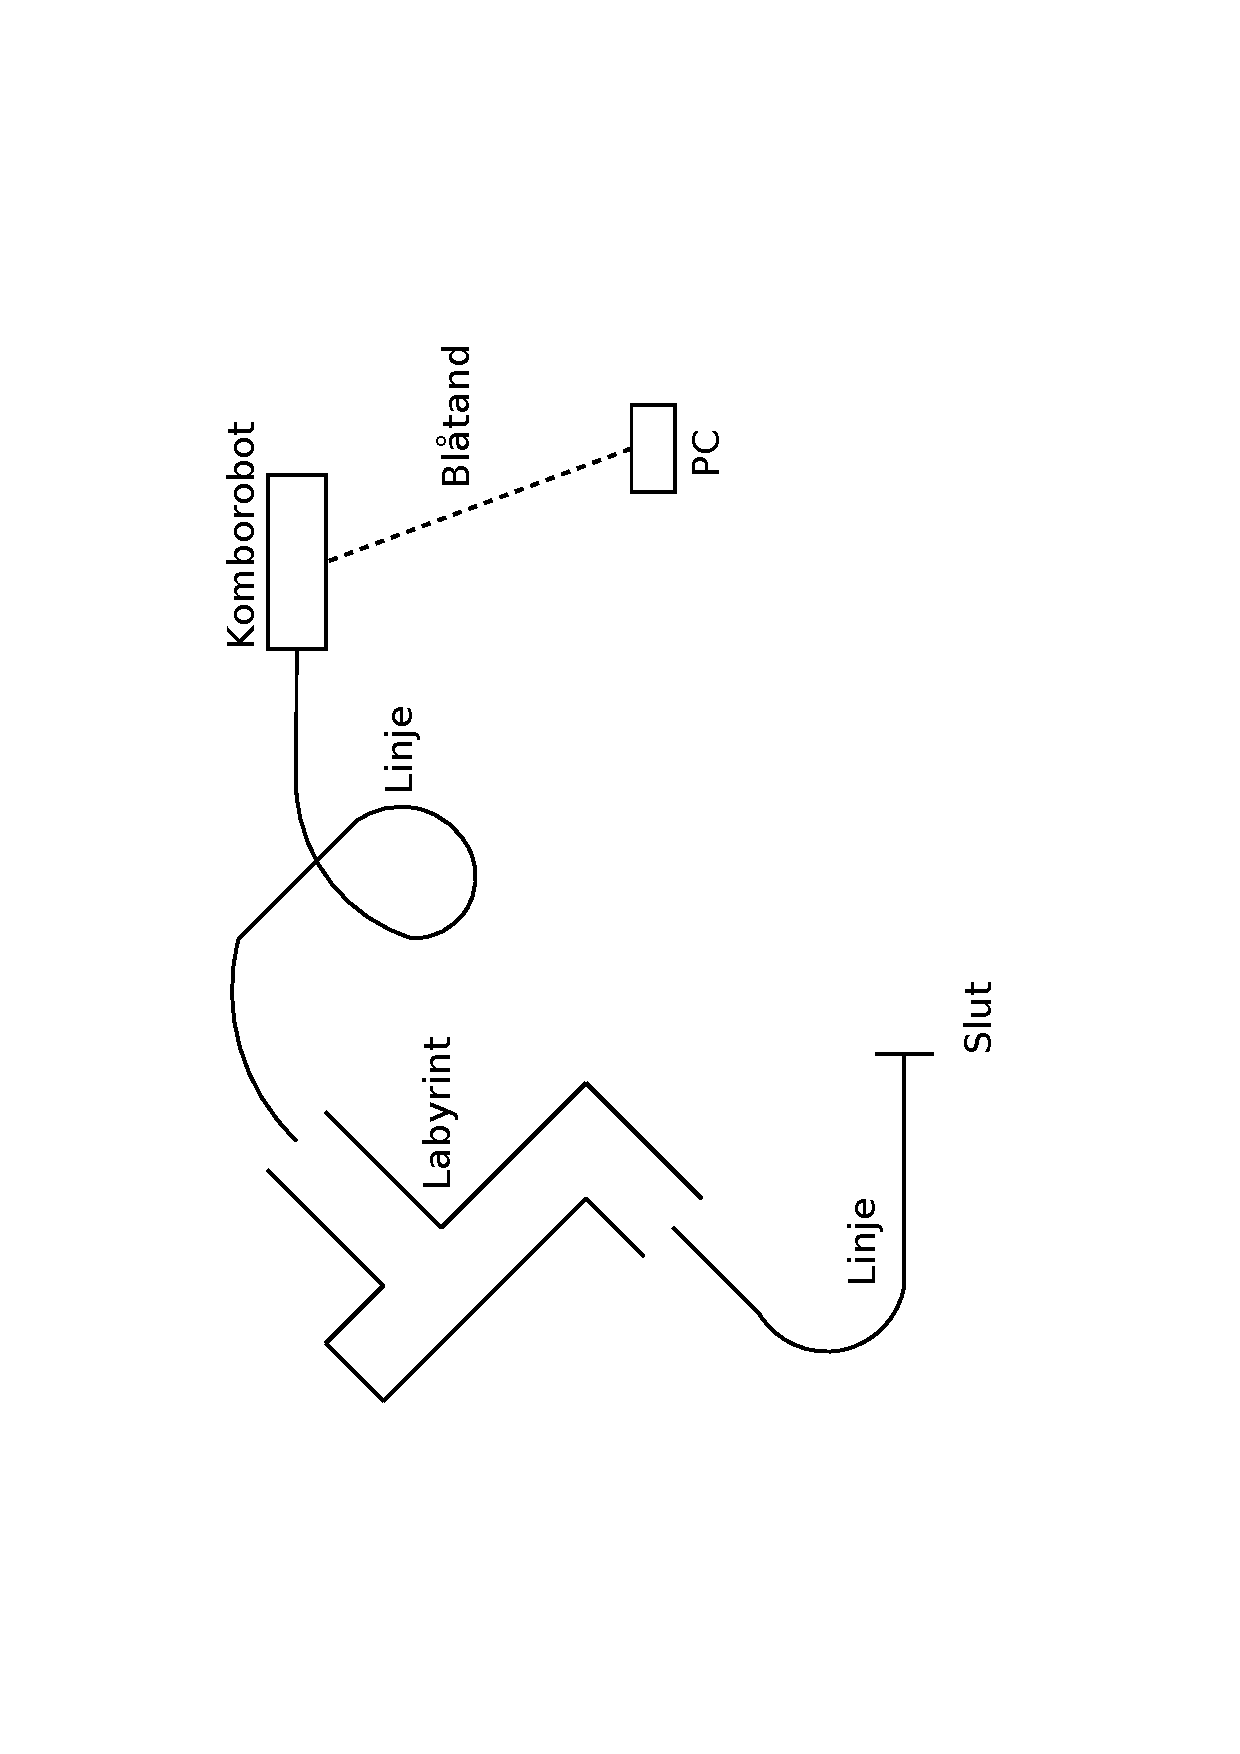
\includegraphics[angle=270,scale=0.5]{Oversikt.pdf}

\section{Översikt av systemet}
På plattformen kommer tre enheter att monteras:
\begin{itemize}
        \item Kommunikationsenhet
        \item Sensorenhet
        \item Styrenhet
Varje enhet kommer styras av en egen AVR-processor.
\subsection{Kommunikation}
De tre enheterna måste kunna kommunicera med varandra, här förslås en I2C-buss och ett system med flera UART.

\subsubsection{I2C}

\end{itemize}
\begin{center}
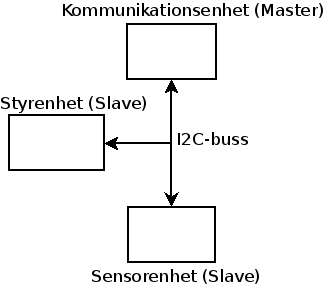
\includegraphics[scale=0.7]{delsystem_i2c.png}
\end{center}
De olika enheterna kommer att kommunicera över en I2C-buss där kommunikationsenheten är master och de andra två enheterna är slave,
detta är för att den mesta kommunikationen kommer att ske genom kommunkationsenheten.

\subsubsection{UART}

\begin{center}
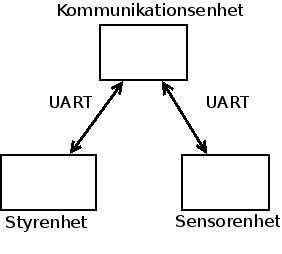
\includegraphics[scale=0.7]{delsystem_uart.png}
\end{center}
De olika enheterna kommer att kommunicera med de i processorerna inbyggda UART-portarna. 
Då dessa redan finns i processorerna blir de lättare att implementera. Det finns dock en nackdel, UART är en 
punkt till punkt kommunikation och då det är tre enheter som måste kommunicera med varandra måste minst en enhet
ha två UART-portar, men processorerna har bara en inbyggd UART-port. Detta går att lösa genom att omvandla en av de generella 
IO-portarna på processorerna till en UART med hjälp av mjukvara. 
Det räcker med att kommunikationsenhten har en extra UART om all kommunikation sker genom den enheten.

\subsection{Uppgraderbarhet}
Ett tydligt kommunikationsprotokoll mellan enheterna kommer att användas så att det är lätt att modifiera enheter.
Om en I2C-buss används blir det lättare at lägga till och byta ut enheter då I2C kan ses som en standardbuss.
Om istället UART används som kommunikation blir det svårare att lägga till nya enheter då flera UART-portar måste implementeras.
Att byta ut eller uppgradera en enhet blir dock lika enkelt med en UART som med en I2C.

PC-mjukavaran kommer att skicka och ta emot data från kommunikationsenheten via blåtand.
Mjukvaran kommer att använda ett tydligt protokoll vilket gör det möjligt att utveckla egen mjukvara eller uppgradera den befintliga mjukvaran.
\section{Delsystem}

\subsection{Kommunkationsenhet}
Kommunikationsenheten ansvarar för att förmedla information mellan de olika
enheterna i systemet. Detta kommer ske via en blåtandslänk mellan en PC och
själva roboten och antingen via en I2C-buss eller UART.

Kommunikationsenheten gör själv inga tolkningar av vad som skickas, den ser bara
till att saker skickas till rätt destination.
\subsubsection{Blåtand}
Kommunikationsenheten kommer via blåtand att kommunicera med en PC och förmedla
instruktioner från PCn till roboten. Kommunikationsenheten kommer dessutom att
skicka information från robotens olika enheter till PCn så att användaren kan få
en uppfattning om vad roboten faktiskt håller på att göra.
\subsubsection{I2C}
Kommunikationsenheten kommer agera master för I2C-bussen, vilket innebär att all
information på bussen kommer gå via kommunikationsenheten. Detta för att
kommunikationsenheten kommer behöva skicka data till samtliga andra enheter från
samtliga enheter.
\subsubsection{UART}
Då en UART används kommer all information att skickas först till
kommunikationsenheten för att sedan därifrfån skickas till rätt destination,
antingen via UART om destinationen är en enhet på roboten eller via blåtand om
destinationen är PCn.


\subsection{Sensorenhet}
Sensorenheten har som uppgift att läsa av omgivningen och beräkna vilken position roboten har relativt mitten av banan och skicka detta vidare till styrenheten. För detta kommer två olika typer av sensorer att behövas, en typ för att läsa linjer och markeringar och en för att bestämma avstånd till väggar.


\subsubsection{Labyrintsensor}
För prioritet 1 behövs två  optiska avståndssensorer placerade på vardera sida om roboten. För prioritetsnivå 2 och 3 kommer en tredje riktad frammåt vara nödvändig. Lämpliga sensorer är de IR sensorer med avstånd på 20 till 150 cm som fungerar för alla prioritetsnivåer, vid prioritetsnivå 1 kan även sensorer med intervallet 10 till 80 cm användas.
Vid korsningar och 90\degree s kurvor kommer avståndet till åtminstonde den ena väggen bli för stort, om det är en korsning skall en riktningsmarkering ha hittats och sparats och styrenheten kan då specialbehandla korsningen. Om ingen markering hittats är det en 90\degree s kurva och sensorenheten signalerar att styrenheten ska köra i den riktning där det inte finns någon vägg som då också måste specialbehandlas av styrenheten.
\begin{center}
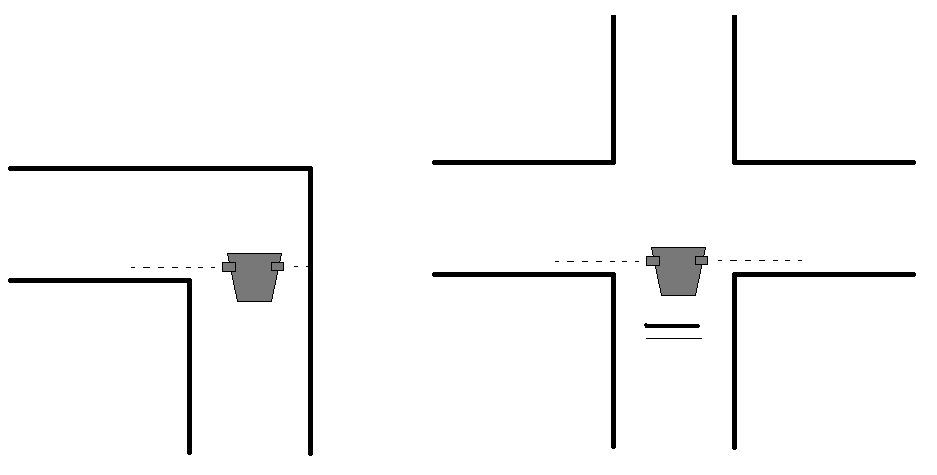
\includegraphics[scale=0.45]{korsningar.png}
\end{center}


Som prioritet 2 skall roboten visa avståndet till väggarna på en display när bilen kör i labyrinten, här finns alternativen LCD-display och alfanumerisk LED-display.

\subsubsection{Linjesensor}
För att upptäcka och läsa av linjer och markeringar på marken kan en reflexsensormodul bestånde av 11 st IR-lysdioder används. Dessa nyttjas genom att en diod tänds, reflektionen A/D omvandlas varefter dioden släcks så att detta kan upprepas på nästa diod. Det avlästa värdet trösklas till tejp eller icke tejp för enkel hantering. 
Linjen får korsa sig själv vilket kommer betyda att alla dioder kan visa tejp, detta bör kunna hanteras igenom att roboten får fortsätta i sin färdriktning tills korsningen passerats.

\subsubsection{Arbetsblock}
Följande arbetsuppgifter finns hos sensorenheten
\begin{itemize}
        \item A/D omvandling
        \item Koda tolkning av avstånd
        \item Koda tolkning av reflexsensormodulens värden
        \item Koda övergången från linjeföljare till labyrintnavigerare
        \item Hantera korsningar och 90\degree s kurvor
        \item Skicka data till styrenheten (via kommunikationsenheten)
\end{itemize}

\subsection{Styrenhet}
Styrenheten kommer att styra motorerna och sköta regleringen så att roboten kan följa en linje och navigera en labyrint utan att slingra sig fram.
När roboten är i fjärrstyrt läge så ska styrenheten ta emot styrkommandon från kommunikationsenheten.
Styrenheten ska sedan styra motorerna så att dessa kommandon utförs. De styrkommandon som ska kunna behandlas är:
\begin{itemize}
        \item Framåt
        \item Fram vänster
        \item Fram höger
        \item Bakåt
        \item Rotera vänster
        \item Rotera Höger
        \item Stopp
\end{itemize}

När roboten är i automatiskt läge (dvs. linjeföljande eller labyrintnavigerande) så ska den ta emot skillnaden mellan aktuellt och önskat läge.
Detta värdet räknas ut av sensorenheten och skickas till styrenheten via kommunikationsenheten.
Utifrån det värdet ska styrenheten reglera motorerna med en PD-regulator. Vissa specialkommandon ska också kunna hanteras i autonomt läge 
för att hantera 90\degree s svängar i labyrinten och korsningar. De specialkommandon som ska kunna hanteras är:
\begin{itemize}
        \item Sväng vänster 90\degree
        \item Sväng höger 90\degree
        \item Kör rakt fram x cm
\end{itemize}

Information om hur styrenheten kör ska skickas till kommunikationsenheten, t ex svänger vänster.

\subsubsection{Arbetsblock}
\begin{itemize}
        \item Ta emot data från kommunikationsenheten
        \item Reglera motorer utifrån sensorvärden
        \item Koda styrkommandon
        \item Koda specialkommandon
        \item Skicka styrinfo till kommunikationsenheten
        \item Implementera alla kommandon
\end{itemize}

\end{document} 

%%% Local Variables: 
%%% mode: latex
%%% TeX-master: t
%%% End: 
